\documentclass[11pt,a4paper]{article}
\usepackage[utf8]{inputenc}
\usepackage{amsmath}
\usepackage{amsfonts}
\usepackage{amssymb}
\usepackage{url}
\usepackage[margin=1.2in]{geometry} %make margins smaller
\usepackage{indentfirst} %to indent the first paragraph

%for figures
\usepackage{graphicx}
\usepackage{wrapfig}
\usepackage{caption}
\captionsetup[figure]{font=small}
\captionsetup{justification=centering}
\usepackage{subcaption}
\usepackage{float}
%\graphicspath{{/home/an20830/Documents/COMPASS/TB2/Mini Project/MSLDA/analysis/}} %Setting the graphicspath

\usepackage{csquotes} %for quotes
\usepackage{booktabs} %for tables
\usepackage[ruled,vlined]{algorithm2e} %for algorithms
\usepackage{hyperref} %for links

\DeclareMathOperator*{\argmin}{argmin}

\begin{document}
\title{Modelling household electricity demand}
\author{Euan Enticott, Georgina Mansell, and Conor Newton}
\date{\today}

\maketitle
 
\section*{Abstract}


\section{Introduction}

\section{Data} \label{data}
A dataset of residential electricity demand was collected as part of a customer behaviour trial in 2010 in Ireland. Electricity consumption was recorded for 2672 households at half hour intervals over the year.

Figure \ref{fig:totalusage} shows the total electricity demand profile for the households. There is a characteristic pattern of low demand at night, a low peak around 7am and a higher peak around 6pm. There are some seasonal effects where demand is higher in the winter months, likely due to increased heating and lighting. The profile also differs on weekends where there is no dip in demand during typical work hours.

\begin{figure}[ht]
\centering
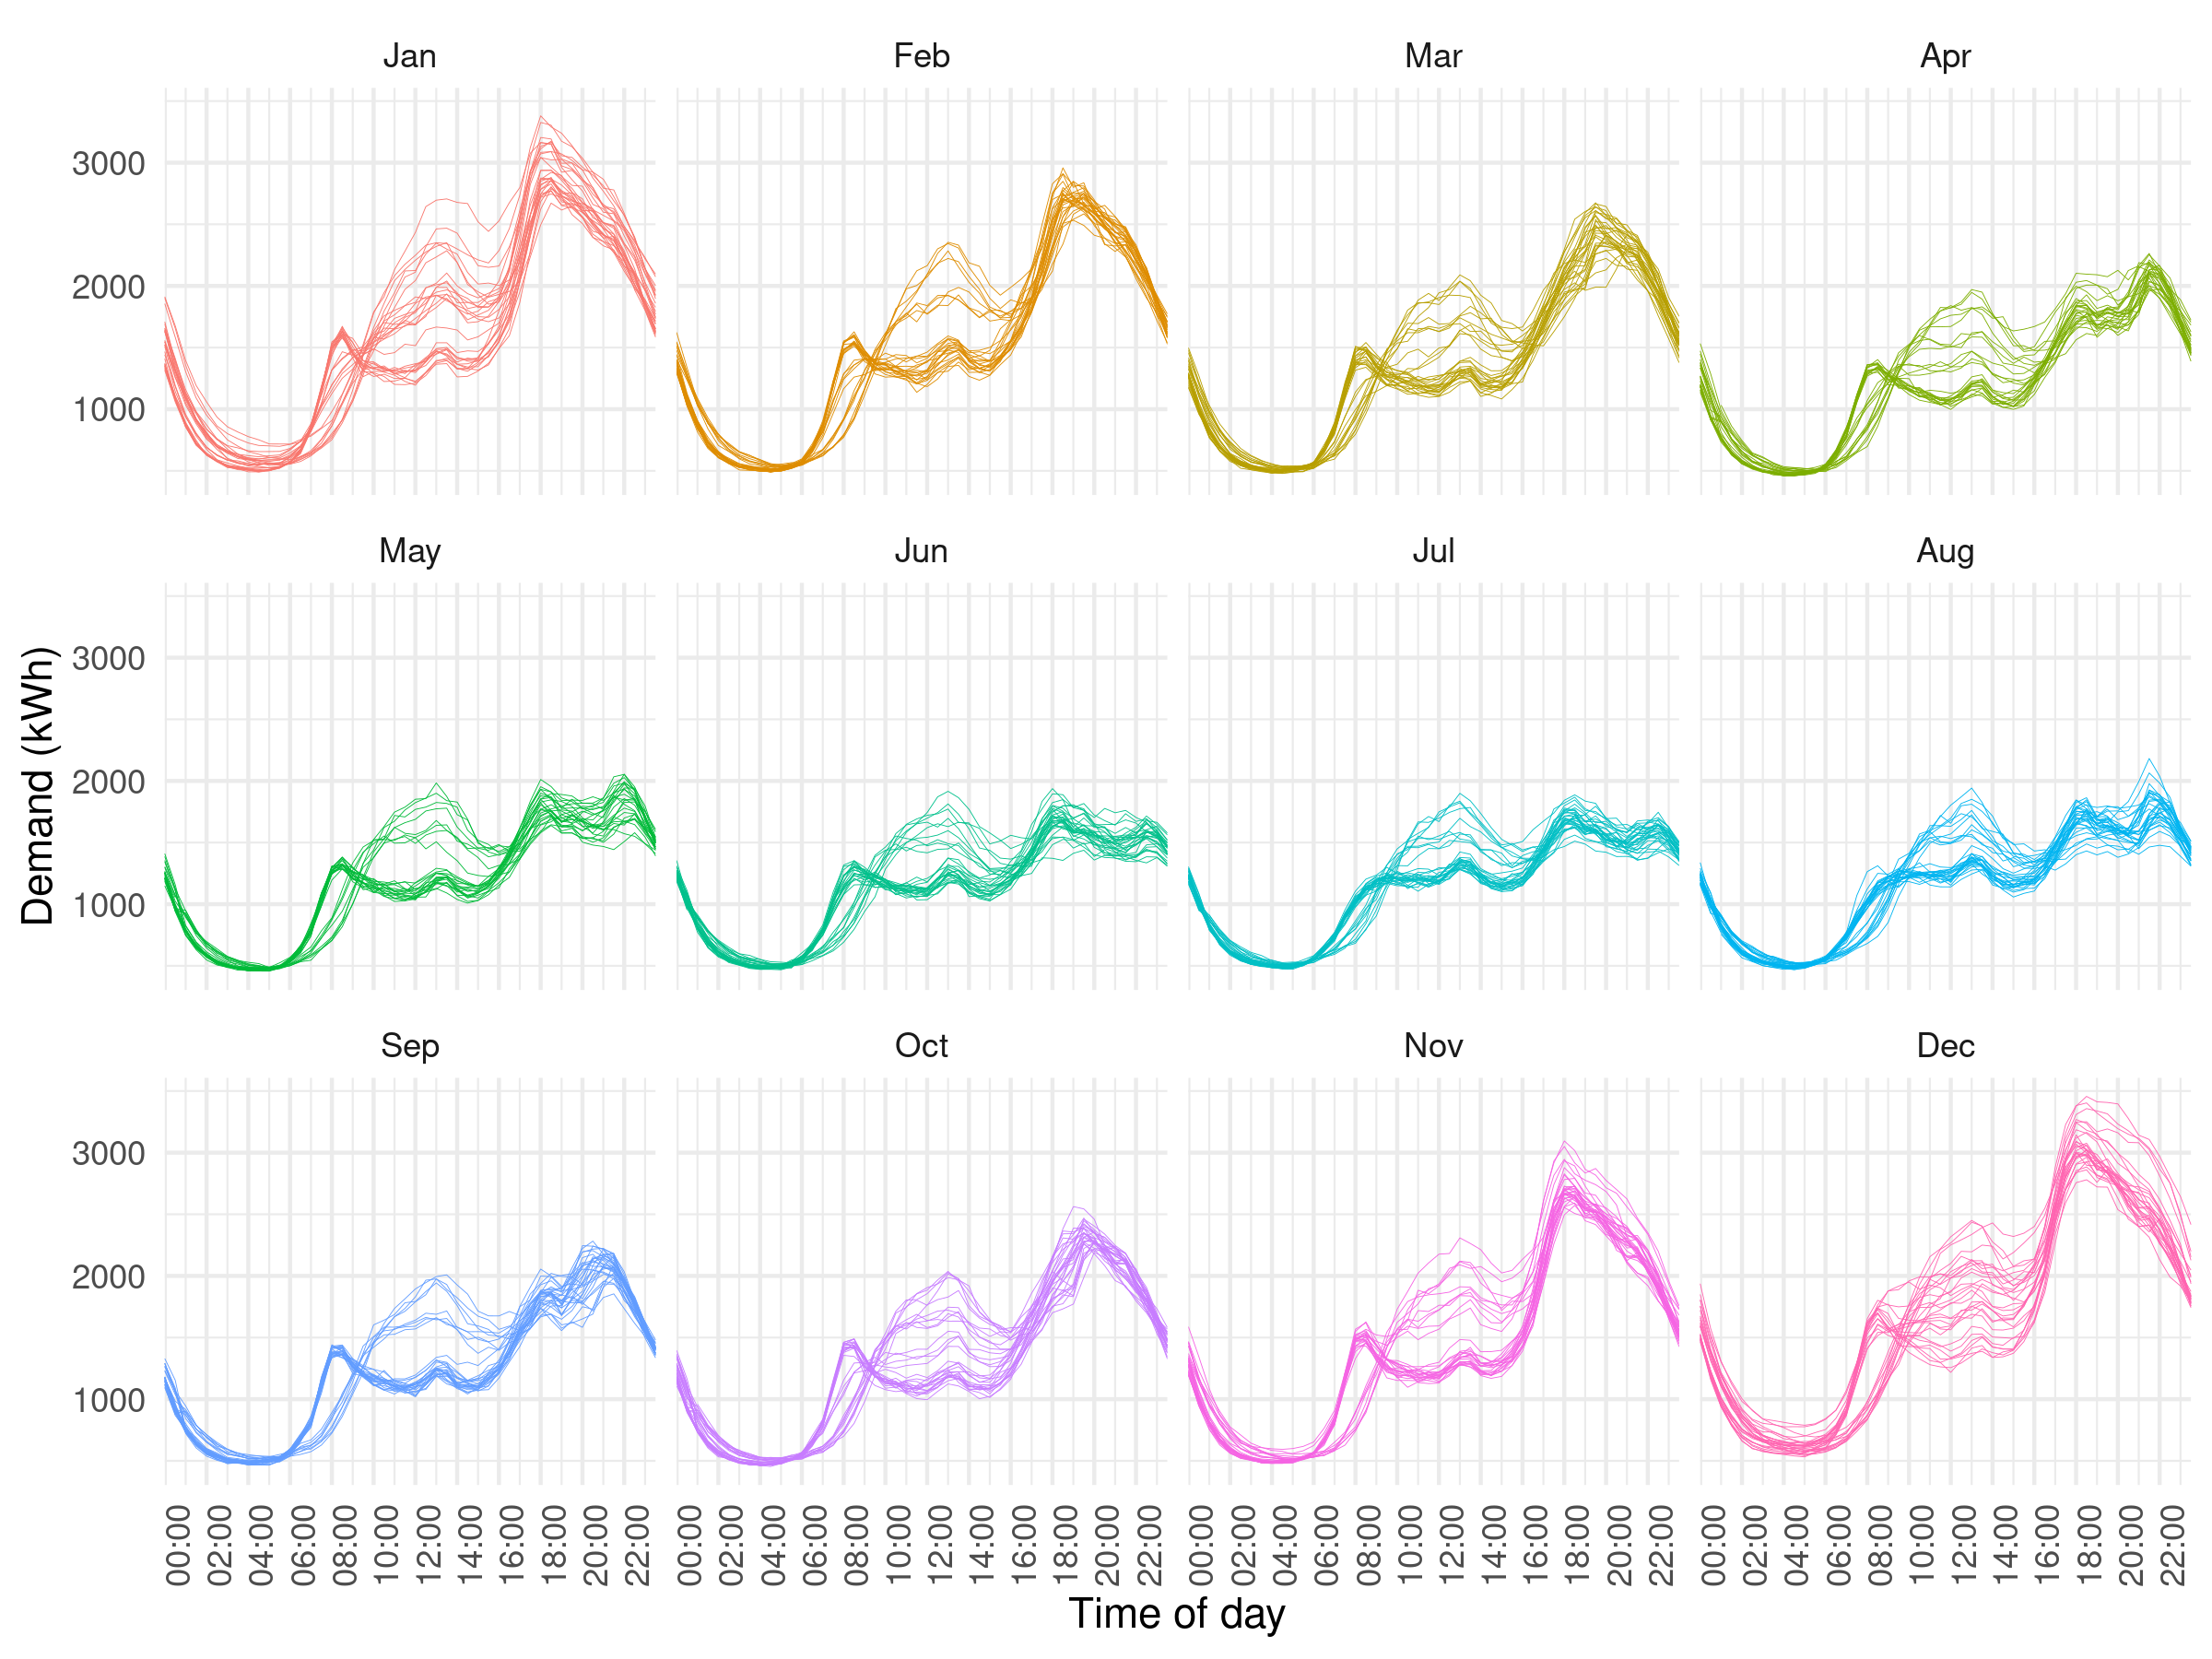
\includegraphics[width=1\linewidth]{TotalUsage}
\caption{Total electricity demand over all recorded households; each line shows the usage over one day, split over subfigures by month.}
\label{fig:totalusage}
\end{figure}

While there is a very clear pattern to the demand at an aggregated level, individual customer profiles are much more varied.

The dataset comes with additional information such as the external temperature, the year the house was built, and whether the house has electric heating. 

The dataset is available at \url{https://github.com/mfasiolo/electBook/blob/master/data/Irish.RData}, and more information about the original study can be found at \url{http://www.ucd.ie/issda/data/commissionforenergyregulationcer/}.

\section{Methods} \label{methods}
All code is available on GitHub at \url{github.com/eenticott/electricity-modelling}.

\subsection{Clustering}

\subsection{Ridge Regression} 
Ridge regression is a commonly used regularisation technique for least squares regression. 
In the standard setting we have a dataset of $n$ samples each with a vector of $p$ covariates $\textbf{x}_i$ and scalar response $y_i$. 
%$\mathcal{D} = \{\textbf{x}_i, y_i\}_{i=1}^n$.
The terms are collected in design matrix $\textbf{X} \in \mathcal{R}^{n \times p}$ and response vector $\textbf{y} \in \mathbb{R}^n$. Typically the matrix $\textbf{X}$ is standardised so that each variable has a zero mean and unit variance. 

Ordinary least squares aims to find the vector of parameters $\beta \in \mathbb{R}^p$ which minimises the residual sum of squares:
$$\hat{\beta} = \argmin_{\beta} || \textbf{y} - \textbf{X} \beta ||^2$$

However, OLS is susceptible to over-fitting; as the number of variables $p$ increases, so does the model variance. Additionally, if $p>n$ or if there is multicollinearity between variables, the matrix $\textbf{X}^T\textbf{X}$ is not invertible. 

Ridge regression can overcome both of these issues by placing an $L_2$ penalty term on the parameter vector $\beta$:
$$\hat{\beta} = \argmin_{\beta} || \textbf{y} - \textbf{X} \beta ||^2 + \lambda ||\beta||^2$$

Here $\lambda \geq 0$ is a hyperparameter which controls the strength of the regularisation and which should be selected through a cross validation procedure. 

Solving for $\beta$ analytically gives: 
$$\hat{\beta} = (\lambda \textbf{I} + \textbf{X}^{\top} \textbf{X})^{-1} \textbf{X}^{\top}\textbf{y}$$

 
- Ridge regression with factor variables?


\subsection{Selecting \texorpdfstring{$\lambda$}{l}}
A simple way to select lambda is to calculate the mean square error on a held out portion of the dataset, then select the value of $\lambda$ which minimises the MSE. An approach that is less sensitive to the specific choice of test data is leave-one-out cross validation (OCV). This is calculated as:

$$\text{OCV} = \frac{1}{n} \sum_{i=1}^n \left( y_i - \hat{\mu}_i^{[-i]} \right)^2$$

OCV can also be re-written as:
$$\text{OCV} = \frac{1}{n} \sum_{i=1}^n \frac{(y_i - \hat{\mu})^2}{(1-A_{ii})^2}$$
which is less computationally expensive, as only one model needs to be fit per $\lambda$, not $n$.

- GCV is apparently better?
 
\subsection{Bayesian Perspective}
Ridge regression can also be considered from a Bayesian perspective; we assume that the responses $y$ are generated by the following process:
$$y = \beta \textbf{x} + \epsilon \quad \text{where} \quad \epsilon \sim \mathcal{N}(0, \sigma^2)$$

Equivalently
$$ \textbf{y} \sim \mathcal{N}(\textbf{X} \beta, \textbf{I} \sigma^2) $$

We could t
 

\subsection{R Package} 


\begin{algorithm}[H] \label{alg1}
\DontPrintSemicolon
\SetAlgoLined
\KwData{...}
\KwResult{...}
Text\;
\Repeat{convergence}{
	$a=b$
}
\For{i=1, 2, ...}{
	Initialise $b$ \;
	$a=b$}
\caption{Algorithm1}
\end{algorithm}


\section{Results}

\section{Conclusion}

%\pagebreak
%\bibliographystyle{ieeetr}
%\bibliography{Citations}

%start appendix and number equations A.1
%\pagebreak
%\appendix
%\numberwithin{equation}{section} 

\end{document}